The focus of the stepped solver is helping a user understand how each algorithm reaches a solution. Therefore we move the configuration panel to a modal window (\cref{fig:step_sol_modal}) to make room for a new panel to describe each step of the algorithm.

%TC:ignore
\begin{figure}[H]
    \centering
    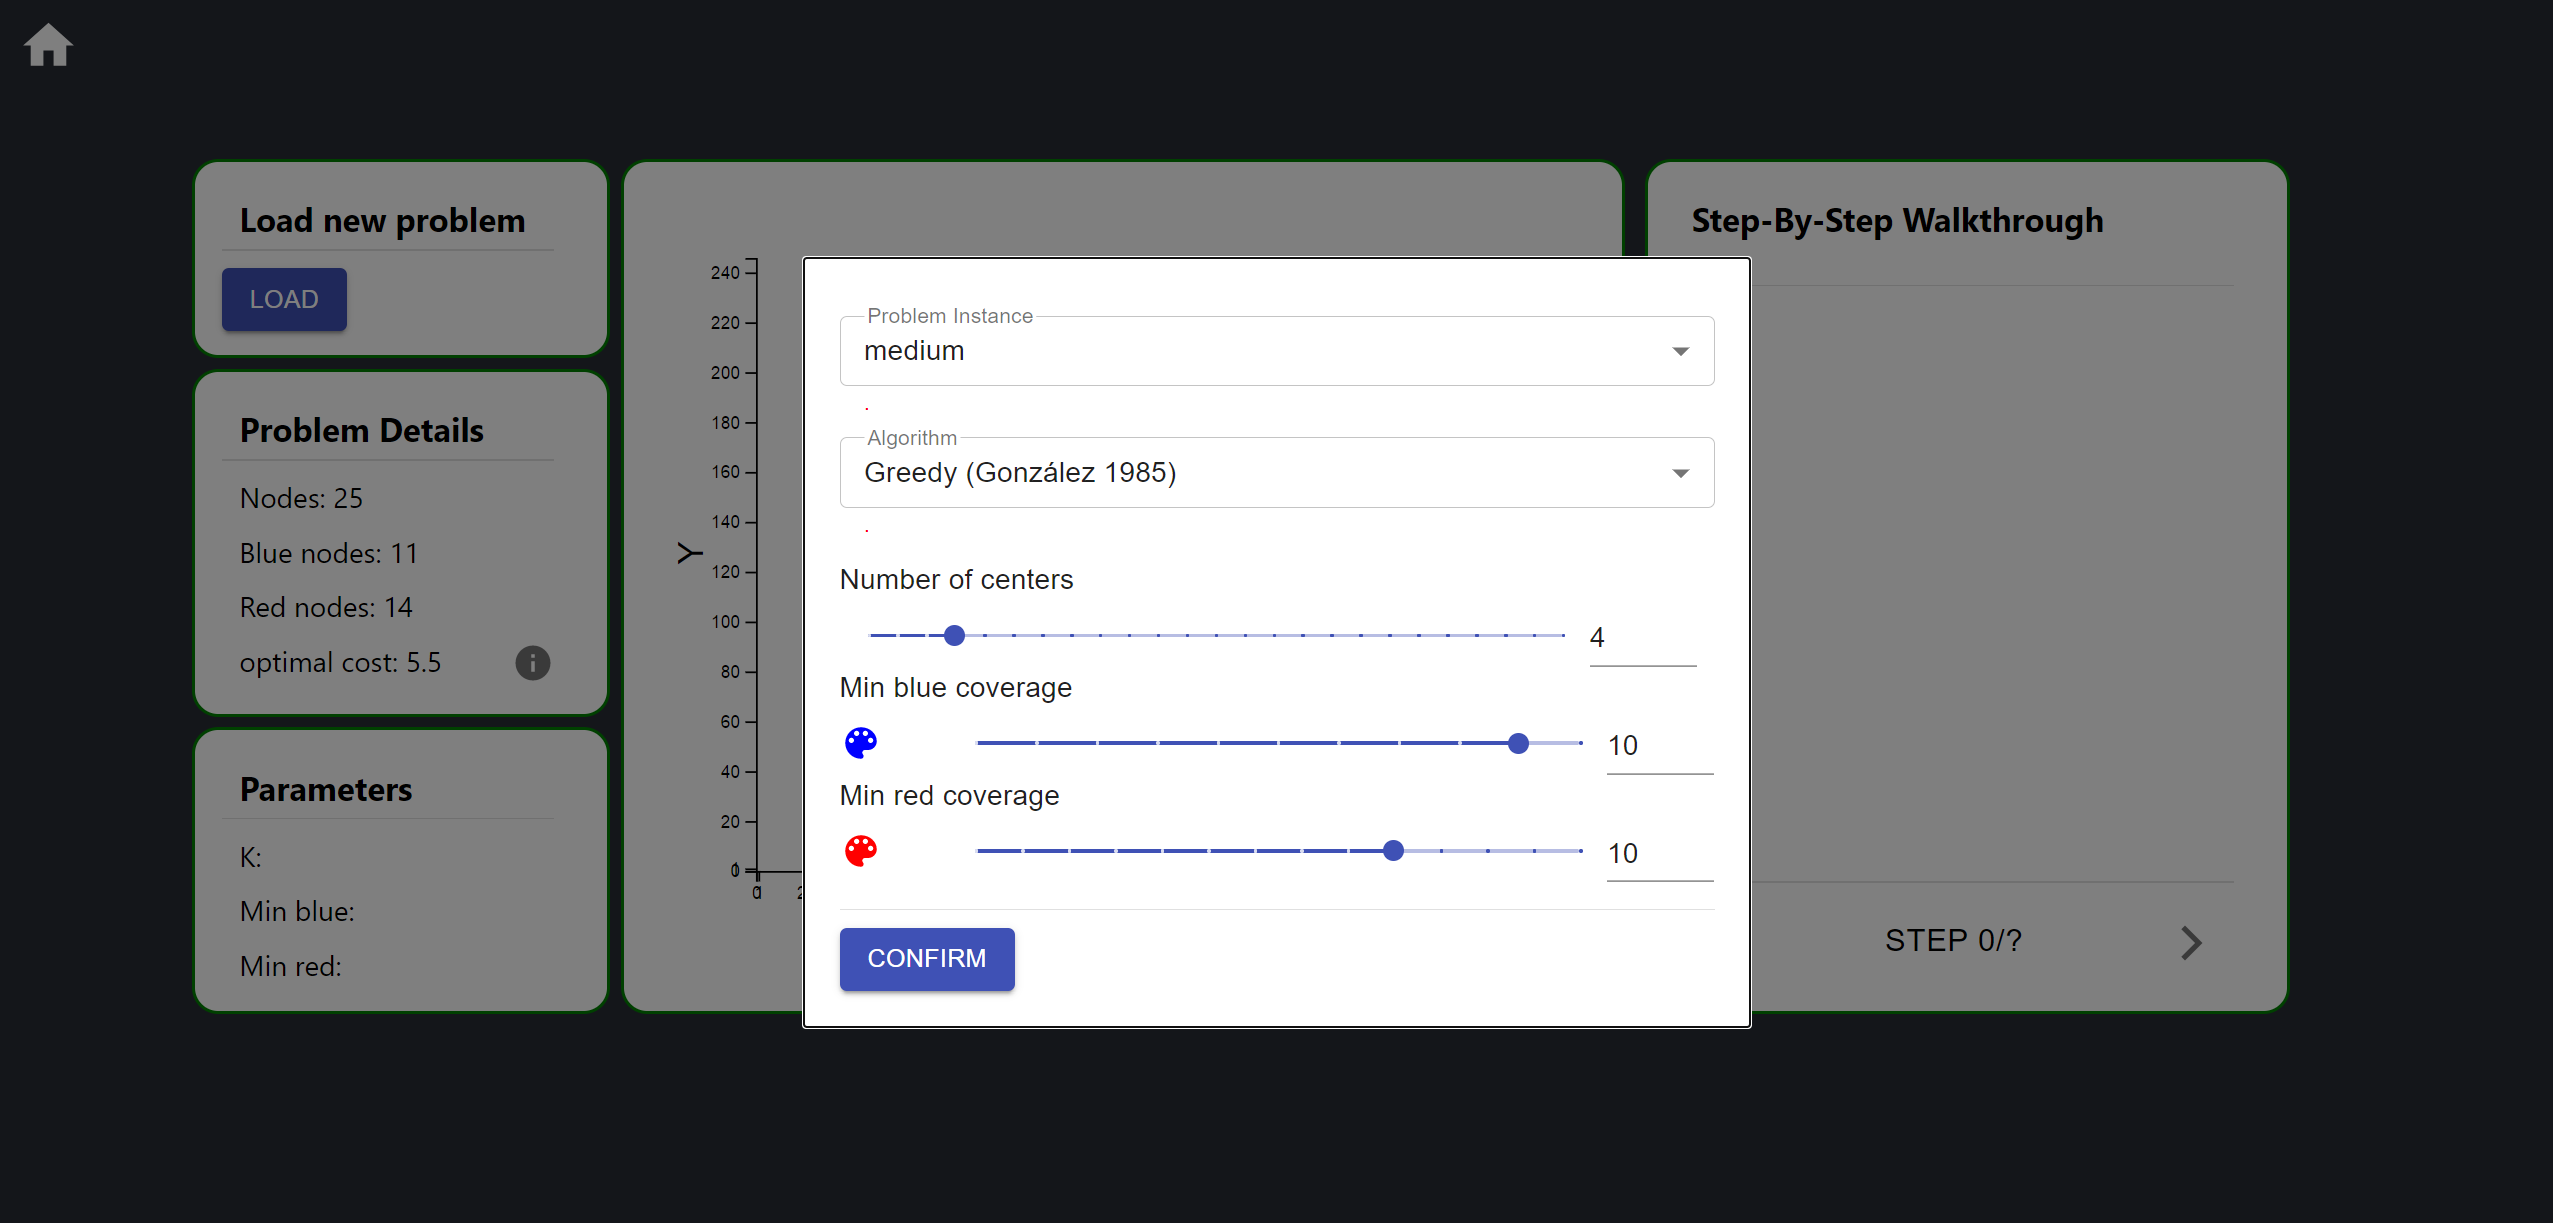
\includegraphics[width=0.7\textwidth]{images/stepped_solver_ui/stepped_solver_modal.png}
    \caption{Stepped Visualisation (configuration modal)\\\url{https://colourful-k-center.herokuapp.com/steps}}
    \label{fig:step_sol_modal}
\end{figure}
%TC:endignore

%TC:ignore
\begin{figure}[H]
    \centering
    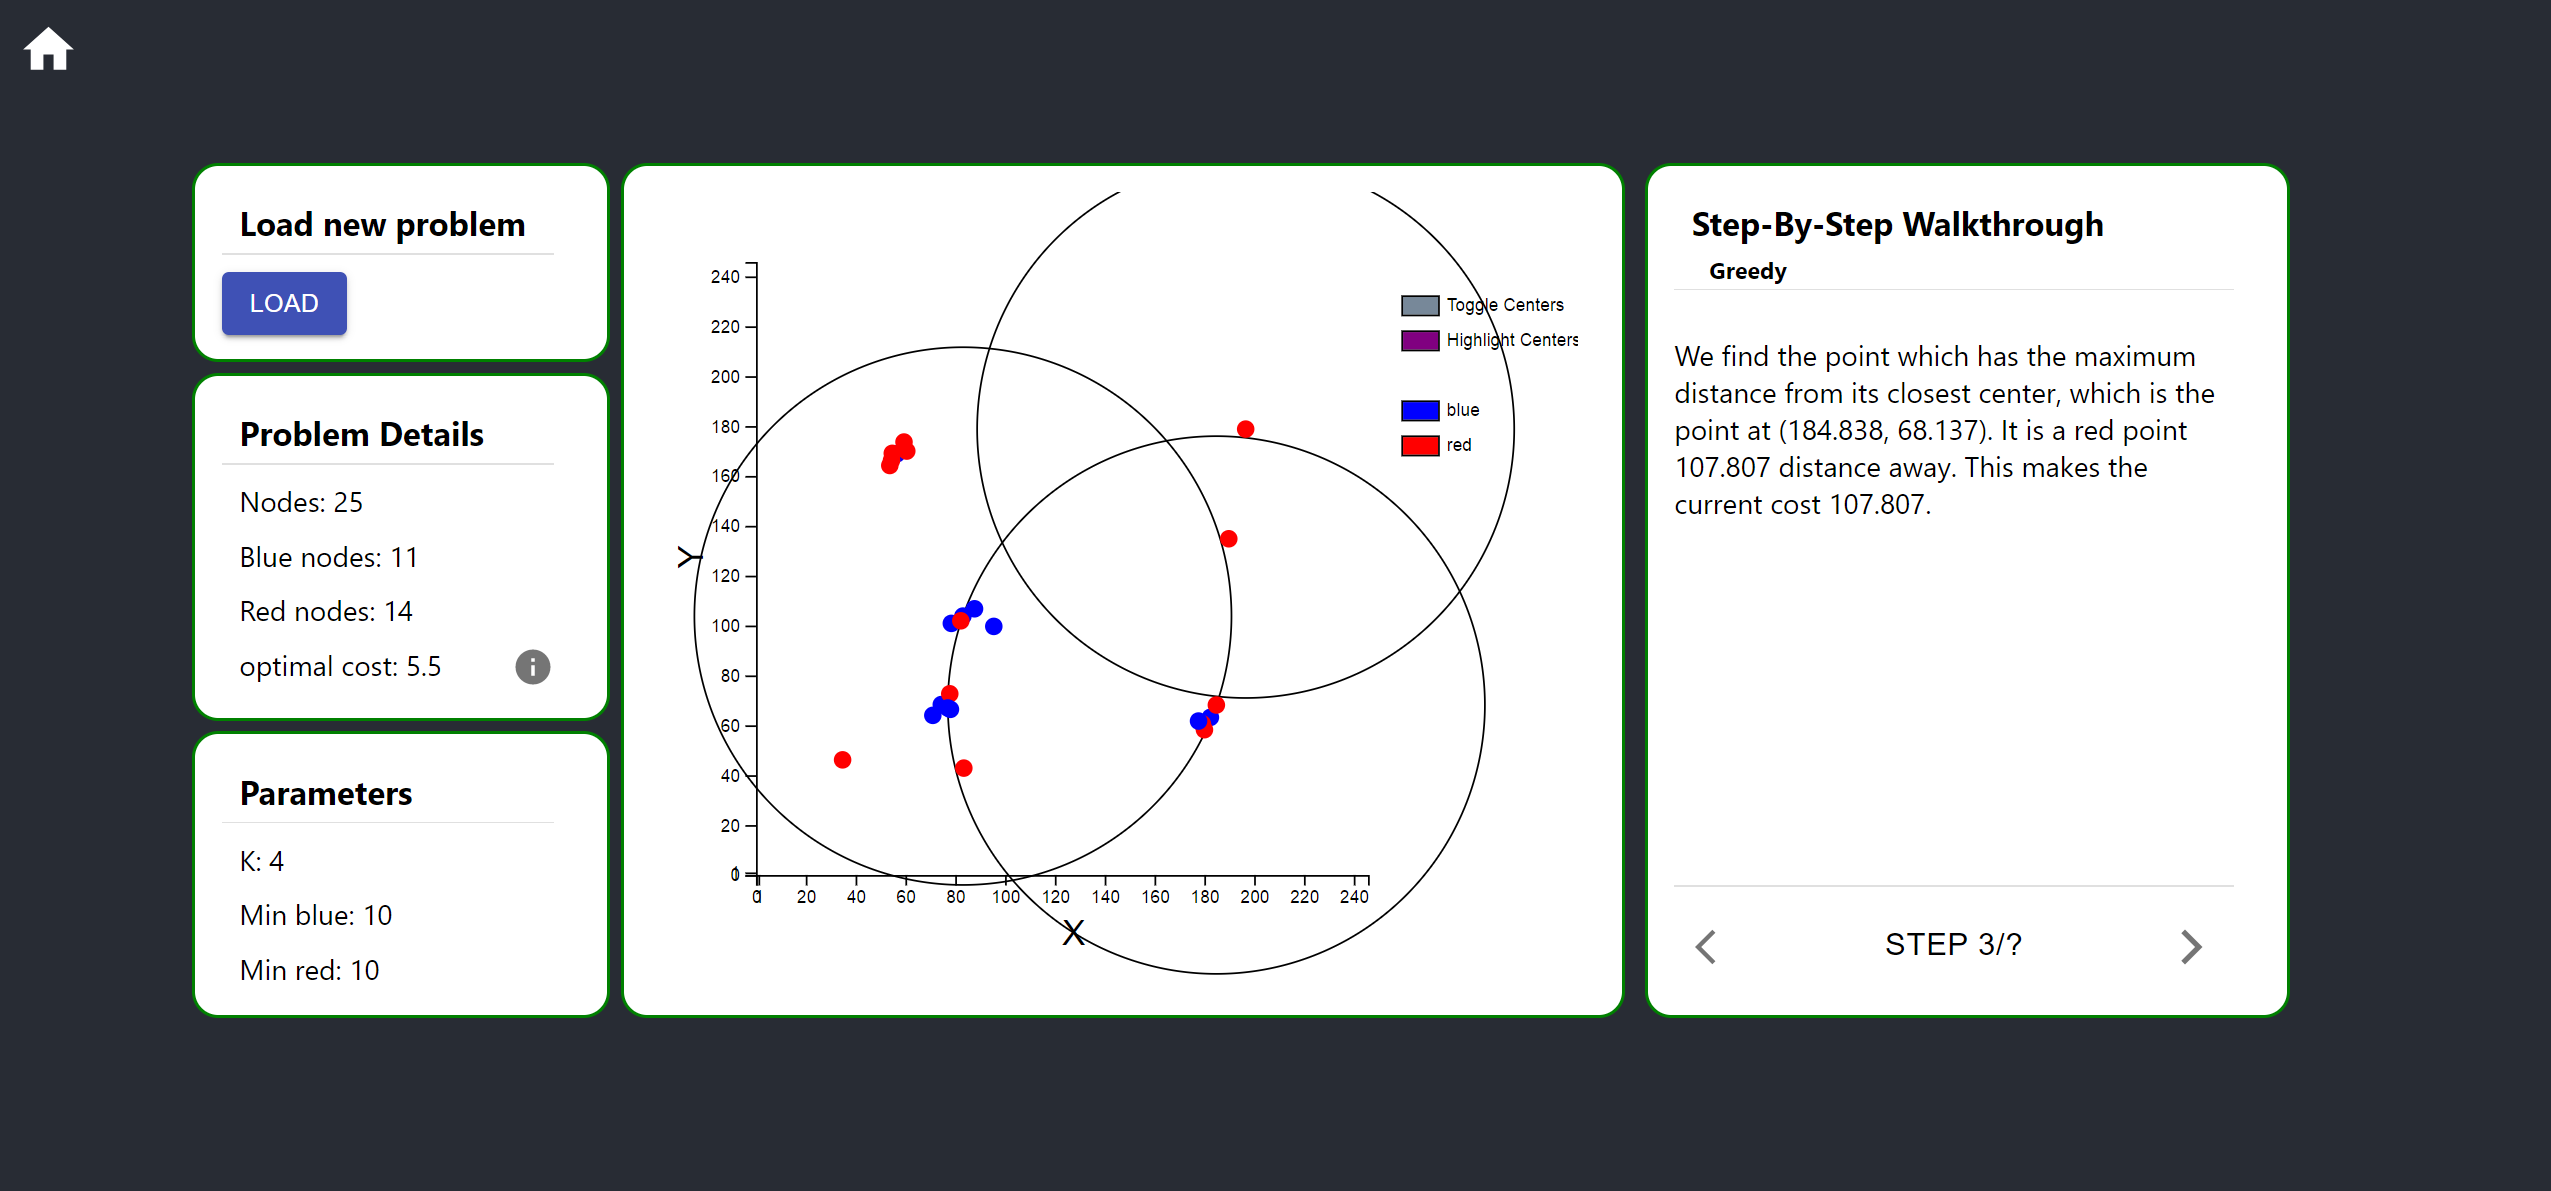
\includegraphics[width=\textwidth]{images/stepped_solver_ui/stepped_solver_greedy.png}
    \caption{Stepped Visualisation\\\url{https://colourful-k-center.herokuapp.com/steps}}
    \label{fig:step_sol_greedy}
\end{figure}
%TC:endignore

Some features of the UI have already been described in \cref{section:solution_visualisation}, therefore we will focus on the differences. We add a walk-through panel (rightmost panel, \cref{fig:step_sol_greedy}) which gives a text description of what an algorithm is doing at the current step. The previous and forward buttons allow the user to traverse the history of algorithm execution on a problem instance. The forward button requests the next step from the server, the exact logic is shown in \cref{fig:step_sol_logic}.

%TC:ignore
\begin{figure}[H]
    \centering
    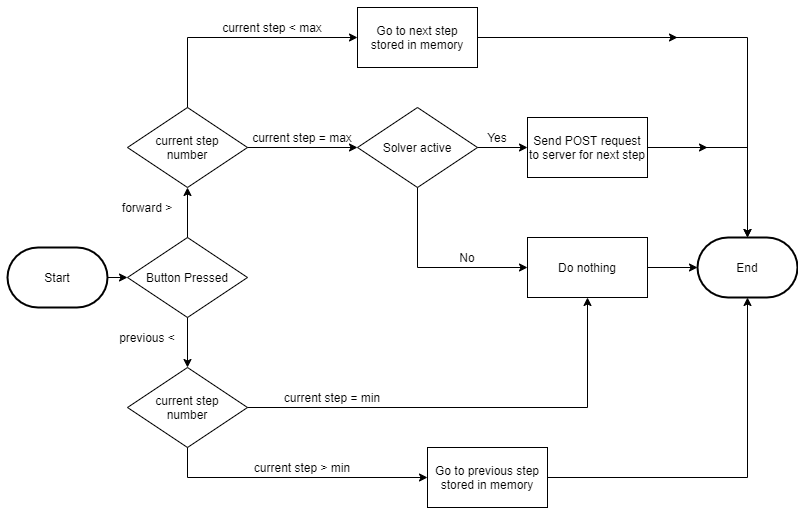
\includegraphics[width=0.85\textwidth]{images/stepped_solver_ui/walkthrough_flow.png}
    \caption{Stepped Visualisation Flow (client side)}
    \label{fig:step_sol_logic}
\end{figure}
%TC:endignore

We make considerations for visualising genetic algorithms (\acrshort{ga}s) since they have multiple solutions at each step. For a \acrshort{ga}, we design a switchable \acrshort{ui}, to show the whole population and a specific individual in the population (\cref{fig:step_sol_toggle}). 

%TC:ignore
\begin{figure}[H]
    \centering
    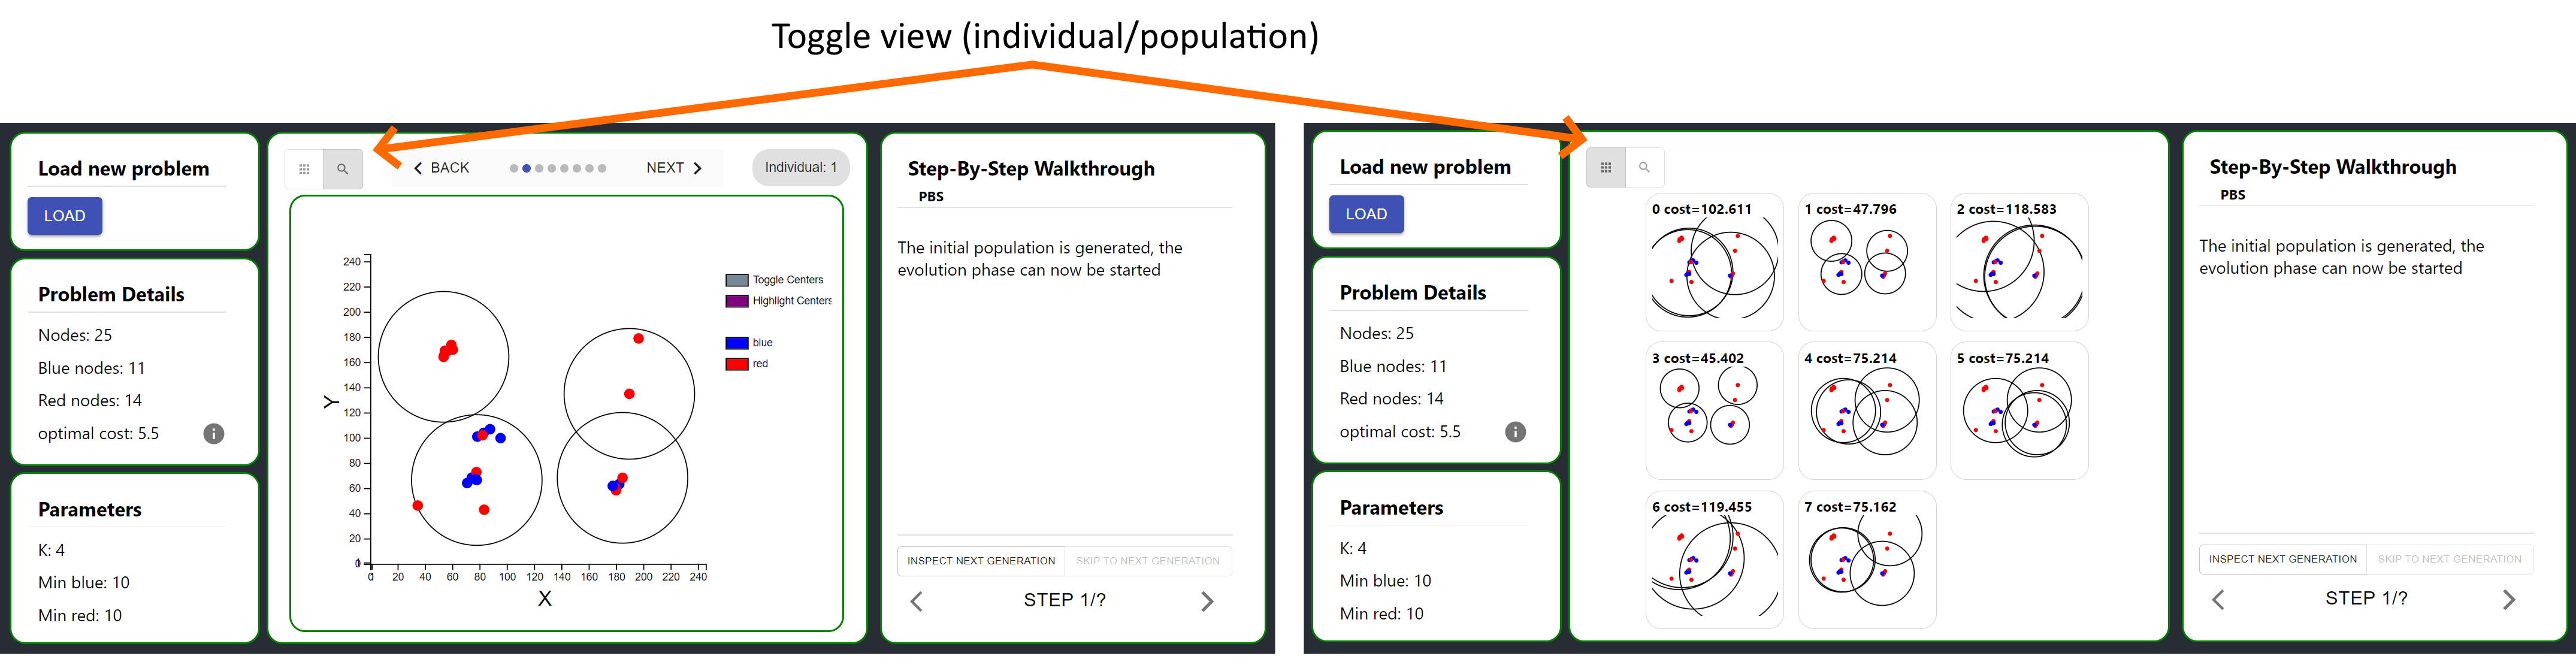
\includegraphics[width=\textwidth]{images/stepped_solver_ui/stepped_solver_toggle.png}
    \caption{View toggling for genetic algorithms}
    \label{fig:step_sol_toggle}
\end{figure}
%TC:endignore

We also consider the large number of steps in \acrshort{ga}s, therefore add an extra control bar to view all steps of the generation or to skip to the next (\cref{fig:step_sol_skip})

%TC:ignore
\begin{figure}[H]
    \centering
    
\includegraphics[width=0.35\textwidth]{images/stepped_solver_ui/stepped_solver_skip.png}
    \caption{Additional controls for genetic algorithms (walk-through panel)}
    \label{fig:step_sol_skip}
\end{figure}
%TC:endignore